% Part: model-theory
% Chapter: interpolation
% Section: separation

\documentclass[../../../include/open-logic-section]{subfiles}

\begin{document}

\olfileid[pt]{mod}{int}{sep}

\olsection{Separação de \printtoken{P}{sentence}}

Precisamos de alguma preparação antes de prosseguir com a demonstração
do teorema da interpolação. Um interpolante para $!A$ e $!B$ é
!!a{sentence}~$!C$ tal que $!A \Entails !C$ e $!C \Entails !B$. Por
contraposição, esta última relação vale se, e somente se,
$\lnot !B \Entails \lnot !C$. Dizemos que !!^a{sentence}~$!C$ com essa
propriedade \emph{separa} $!A$ e $\lnot !B$. Assim, encontrar um
interpolante para $!A$ e $!B$ equivale a encontrar !!a{sentence} que
separe $!A$ e $\lnot !B$. Como tantas vezes ocorre, será útil
considerar uma generalização: uma sentença que separa dois
\emph{conjuntos} de !!{sentence}s.

\begin{defn}
Uma sentença $!C$ \emph{separa} os conjuntos de sentenças $\Gamma$ e
$\Delta$ se, e somente se, $\Gamma \Entails !C$ e $\Delta \Entails
\lnot !C$. Se não existe tal !!{sentence}, então $\Gamma$ e $\Delta$
são \emph{inseparáveis}.
\end{defn}

As relações de inclusão entre as classes de modelos de $\Gamma$,
$\Delta$ e $!C$ são representadas abaixo:
\begin{figure}[h]
  \centering
  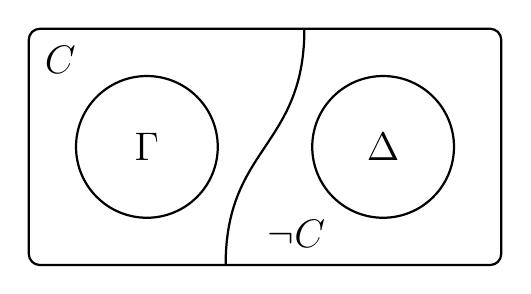
\begin{tikzpicture}[node distance=2cm, auto, thick]
    \draw [rounded corners] (0,0) -- (6,0) -- (6,3) -- (0,3) --  cycle;
    \draw (1.5,1.5) circle (0.9cm);
    \draw (4.5,1.5) circle (0.9cm);
    \path node at (1.5,1.5) {\Large $\Gamma$}; 
    \path node at (4.5,1.5) {\Large $\Delta$}; 
    \path node at (0.4,2.6) {\Large $\formula{C}$};
    \path node at (3.4,0.4) {\Large $\lnot \formula{C}$};
    \draw (2.5,0) .. controls (2.5,1.5) and (3.5,1.5) .. (3.5,3);
  \end{tikzpicture}
  \caption{$!C$ separa $\Gamma$ e $\Delta$}
  \ollabel{fig:sep}
\end{figure}


\begin{lem}\ollabel{lem:sep1}
Suponha que $\Lang{L}_0$ seja a linguagem que contém toda
!!{constant}, !!{function} e !!{predicate} (exceto $\doteq$) que ocorre
\emph{tanto} em $\Gamma$ quanto em $\Delta$, e obtenha $\Lang{L}'_0$
acrescentando infinitas novas !!{constant}s $\Obj c_n$ para $n \ge 0$.
Se $\Gamma$ e $\Delta$ são inseparáveis em $\Lang{L}_0$, então também
são inseparáveis em $\Lang{L}'_0$.
\end{lem}

\begin{proof}
Procedemos indiretamente: suponha, para obter uma contradição, que
$\Gamma$ e $\Delta$ sejam separados em $\Lang{L}'_0$. Então
$\Gamma \Entails \Subst{!C}{c}{x}$ e
$\Delta \Entails \lnot \Subst{!C}{c}{x}$ para algum
$!C \in \Lang{L}_0$ (onde $c$ é uma nova !!{constant}---o caso em que
$!C$ contém mais de uma nova !!{constant} desse tipo é semelhante).
Pela compacidade, existem subconjuntos \emph{finitos} $\Gamma_0$ de
$\Gamma$ e $\Delta_0$ de $\Delta$ tais que
$\Gamma_0 \Entails \Subst{!C}{c}{x}$ e
$\Delta_0 \Entails \lnot \Subst{!C}{c}{x}$. Seja $!G$ a conjunção de
todas as !!{formula}s em $\Gamma_0$ e $!H$ a conjunção de todas as
!!{formula}s em $\Delta_0$. Então
\begin{align*}
  !G & \Entails \Subst{!C}{c}{x}, & !H  \Entails \lnot \Subst{!C}{c}{x}.
\end{align*}
Da primeira relação, por Generalização, obtemos
$!G \Entails \lforall[x][!C]$; da segunda, por contraposição, obtemos
$\Subst{!C}{c}{x} \Entails \lnot !H$, donde também
$\lforall[x][!C] \Entails \lnot \delta$. Outra contraposição fornece
$!H \Entails \lnot \lforall[x][!C]$. Por monotonicidade,
\begin{align*}
  \Gamma &\Entails \lforall[x][!C], & 
  \Delta & \Entails \lnot \lforall[x][!C],
\end{align*}
de modo que $\lforall[x][!C]$ separa $\Gamma$ e $\Delta$ em
$\Lang{L}_0$.
\end{proof}

\begin{lem}\ollabel{lem:sep2}
Suponha que $\Gamma \cup \{ \lexists[x][!S] \}$ e $\Delta$ sejam
inseparáveis e que $c$ seja uma nova !!{constant} que não ocorre em
$\Gamma$, $\Delta$ nem em $!S$. Então
$\Gamma \cup \{ \lexists[x][!S], \Subst{!S}{c}{x} \}$ e $\Delta$
também são inseparáveis.
\end{lem}

\begin{proof}
Suponha, para obter uma contradição, que $!C$ separe
$\Gamma \cup \{ \lexists[x][!S], \Subst{!S}{c}{x}\}$ e $\Delta$,
enquanto $\Gamma \cup \{\lexists[x]{!S} \}$ e $\Delta$ sejam
inseparáveis. Distinguimos dois casos:
\begin{enumerate}
\item $c$ não ocorre em $!C$: nesse caso,
  $\Gamma \cup \{\lexists[x][!S], \lnot!C \}$ é satisfatível (caso
  contrário, $!C$ separa $\Gamma \cup \{\lexists[x][!S] \}$ e
  $\Delta$). O conjunto permanece satisfatível se acrescentarmos
  $\Subst{!S}{c}{x}$, logo, afinal, $!C$ não separa
  $\Gamma \cup \{ \lexists[x][!S], \Subst{!S}{c}{x} \}$ e $\Delta$.
\item $c$ ocorre em $!C$, de modo que $!C$ tem a forma
  $\Subst{!C}{c}{x}$. Então temos
  \[
  \Gamma \cup \{ \lexists[x][!S], \Subst{!S}{c}{x}\} \Entails \Subst{!C}{c}{x},
  \]
  donde $\Gamma, \lexists[x][!S] \Entails
  \lforall[x][(!S \lif !C)]$ pelo Teorema da Dedução e por
  Generalização, e, por fim,
  $\Gamma \cup \{ \lexists[x][!S] \} \Entails \lexists[x][!C]$. Por
  outro lado, $\Delta \Entails \lnot \Subst{!C}{c}{x}$ e, portanto,
  por Generalização, $\Delta \Entails \lnot \lexists[x][!C]$. Logo,
  $\Gamma \cup \{\lexists[x][!S] \}$ e $\Delta$ são separáveis, uma
  contradição.
\end{enumerate}
\end{proof}

\end{document}
